\section{Global Motion Estimation}
\label{sec:02-gme}
Videos are, at their core, sequences of images called frames; we can spot the motion happening between a given pair of frames by detecting which pixels changed position with respect to that pair of frames.

This information can be encoded in a human-understandable format by presenting the \textit{needle diagram} of the two frames; this kind of representation is shown in \cref{fig:needle-diagram}.

\begin{figure}
    \centering
    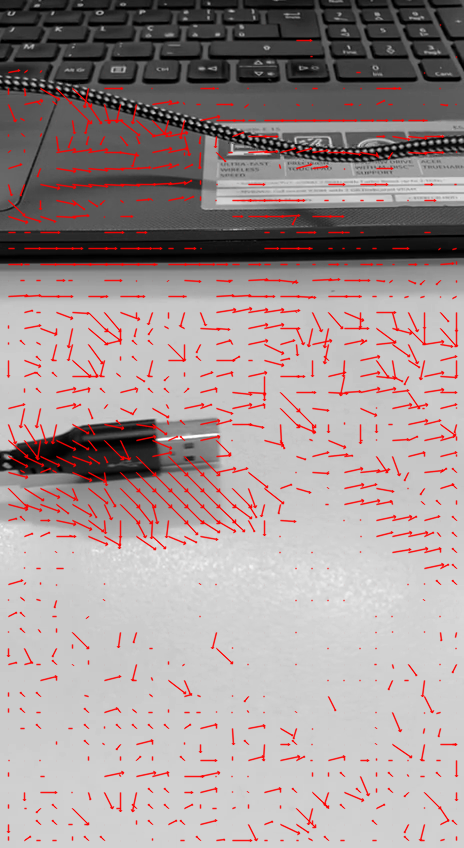
\includegraphics[width=.7\linewidth]{../assets/images/bbme-0-res.png}
    \caption{Needle diagram between two frames of a video sequence.}
    \label{fig:needle-diagram}
\end{figure}

It is pretty clear what information this figure is conveying: for each couple of frames we mark with an arrow the shift that the pixel has made. This gives us an indication of the actual movement of the recorded objects.

However, the motion that we are able to extract from the two frames is what is usually called "apparent motion", which is a combination of two different factors:
\begin{itemize}
    \item the global motion, which corresponds to the motion of the camera;
    \item the effective motion of the objects recorded.
\end{itemize}

An important task in computer vision is the global motion estimation, which aims to distinguish these two different types of motion.
In particular, this information is highly important for a number of applications, amongst which we find video coding, motion compensation, object segmentation and egomotion estimation.

The task of distinguishing which movement is to be classified as global motion and which one is to be classified as object motion instead is not so easy. In fact, there is no clear feature that distinguishes the moving objects from the static background, and this leads to the need for complex tools to differentiate the two types of motion.

% Therefore, to model motion we usually assign to each pixel a vector which describes the shift in the coordinates of that pixel. 

\subsection{Motion Models}
\label{sec:motion-models}

The main approach to global motion estimation consists in using a motion model to describe the motion of the camera.

% What is a motion model?
Motion models describe the motion of the entire visual field through an equation. Basically, the underpinning idea is to write an equation which, given a pixel in a certain position $(x,y)$, returns the position that the same pixel will have in the next frame, if its motion is due only to camera motion.

There is a number of motion models that can be used to describe global motion, ranging from very simple translational models - that can describe only translation motion - to more complex models, allowing to describe pan, tilt, zoom and roll motion patterns. The reader can use as reference \cref{fig:camera-motion} as an illustration of these types of motion.

\begin{figure}
    \centering
    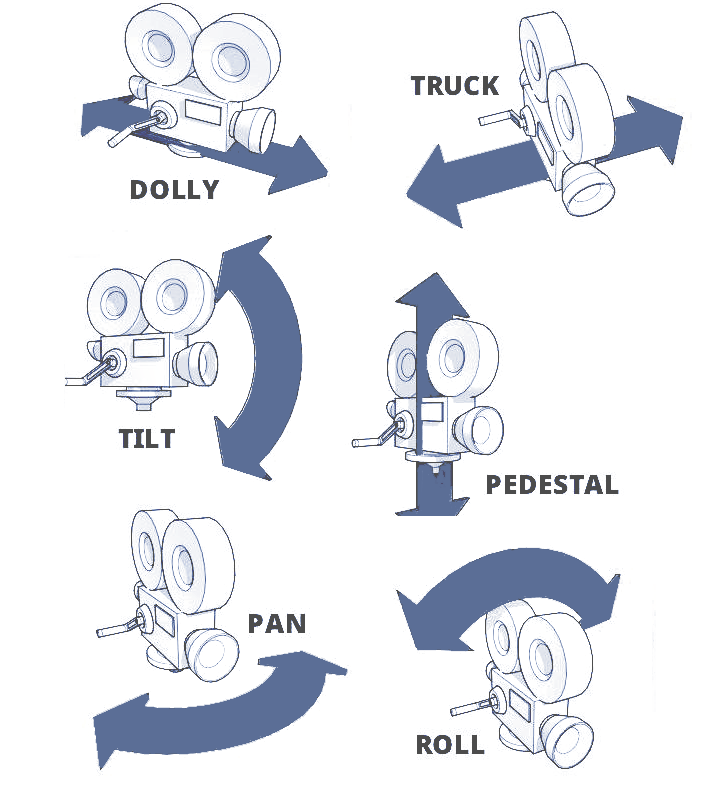
\includegraphics[width=.9\linewidth]{../assets/images/camera-movement.png}
    \caption{Different types of camera motion. Source: \url{https://cinestudy.org/2020/06/29/camera-movement/}.}
    \label{fig:camera-motion}
\end{figure}

All the motion models are defined as functions of some parameters; to get the camera motion in a certain sequence we need to estimate the parameters of the motion model for that precise sequence. Taking as example the motion model we used in this project - the affine motion model - and all the models that describe a rigid motion, the shift in the position of a pixel can be described as in \cref{eq:affine-model-representation}.

\begin{equation}
    \label{eq:affine-model-representation}
    p' = 
    \begin{bmatrix}
        X' \\ Y' \\ Z'
    \end{bmatrix}
    =
    \begin{bmatrix}
        r_1 & r_2 & r_3 \\
        r_4 & r_5 & r_6 \\
        r_7 & r_8 & r_9 
    \end{bmatrix}
    \begin{bmatrix}
        X \\ Y \\ Z
    \end{bmatrix}
    +
    \begin{bmatrix}
        T_X \\ T_Y \\ T_Z
    \end{bmatrix}
    = Rp + T
\end{equation}

Here $p'$ represents the position of the pixel after the camera motion. The matrix $R$ is used to describe rotation and the vector $T$ for the translation component.

The affine motion model can describe simple motions that can be described by linear functions as translation, rotation and zooming (see \cite{Ren20} for in depth explanation).

Usually the affine model is used under the assumptions that the rotation and translation are on the image plane, and that depth $Z$ is approximately constant (as from \cite{WangBook}); these assumptions are reasonable as long as the motion occurring between the two frames we are analyzing is not too large.
Under these assumptions, the affine model can be represented as \cref{eq:affine-model-direct-estimation}, where we need to estimate the 6 parameters $a =[a_1, a_2, a_3, b_1, b_2, b_3 ]$.

\begin{equation}
    \label{eq:affine-model-direct-estimation}
    \begin{split}
        \Delta x &= a_1 x_0 + a_2 y_0 + a_3 \\
        \Delta y &= b_1 x_0 + b_2 y_0 + b_3
    \end{split}
\end{equation}

\subsection{Parameter Estimation}
There are two different approaches to estimate the parameters of a motion model:
\begin{itemize}
    \item a direct approach, which computes the best parameters by optimizing an overdetermined system in the pixel domain;
    \item an indirect approach, which minimizes the approximation error between the motion field obtained with an estimation and the motion field obtained by the motion model.
\end{itemize}

The first approach derives from the equation of the optical flow; in the case of the affine model, it describes the motion of each pixel as in \cref{eq:affine-model-direct-estimation}.
This equation can be applied to any subset of pixels of the frames, therefore the system turns out to be overdetermined and we can solve it using some optimization method, for instance gradient descent.

The second approach - indirect estimation - aims to minimize some error measure between the ground truth motion field and the motion field returned by the motion model.

Therefore, indirect estimation needs, as a preprocessing step, to get the motion field from a motion estimation method - e.g. block-based motion estimation. This motion field is then used as \textit{ground truth} to find the parameters of the motion model that minimize some error measure between this motion field and the one returned by the motion model.

An aspect of this procedure worth highlighting is that it works on the motion field rather than directly on the pixel domain. Hence, it can compute motion of blocks instead of single pixels, reducing the overall complexity of the procedure.

The process is summarized in \cref{eq:indirect-estimation}, where
\begin{itemize}
    \item $a$ is the parameter vector;
    \item $p$ is the single pixel (or block);
    \item $gt(p)$ is the ground truth motion vector for $p$;
    \item $MM(p,a)$ is the motion vector that the motion model would predict for $p$ with parameters $a$;
    \item $E$ is some error measure that accounts for the difference between the two motion vectors, usually a \(p\)-norm distance.
\end{itemize}

\begin{equation}
    \label{eq:indirect-estimation}
    a = \arg \min_a \sum_p E(gt(p) - MM(p, a))
\end{equation}

Once we minimize \cref{eq:indirect-estimation}, we obtain the values of the parameter vector $a$ that encode the camera motion of the video sequence we are analyzing.

\subsection{Robust Estimation}
Since motion in video sequences can be pretty fast and complex, it is often the case that some parts of the scene move in such a way that they insert noise in the motion estimation process.
In particular, it is quite expected to find fast moving objects which we refer to as \emph{outliers}: they are objects manifesting some kind of intrinsic motion - not caused by camera motion - which pollutes the estimation of the parameters of the motion model.

In order to solve this problem, a common approach is to introduce some strategy to remove the outliers from the motion estimation process and, consequently, obtain a robust estimation of the motion field.